%!TEX encoding = UTF-8 Unicode
%!TEX TS-program = pdflatex

%%% --- PREAMBLE --- %%%
\documentclass[a4paper,11pt]{article}

\usepackage[italian]{babel}
\usepackage[left=2cm,right=2cm,top=2cm,bottom=2cm,headheight=14pt]{geometry}
\usepackage[T1]{fontenc} % OT1: basic, T1: western, T3 and T5: exotic, T4: lots of characters but WORSE READABILITY
\usepackage[utf8x]{inputenc} % utf8x supports more characters than utf8
\usepackage{graphicx} % import PNG, JPG and PDF with \includegraphics
\usepackage[usenames,table]{xcolor} % \color
\usepackage{amssymb}
\usepackage{amsmath}
\usepackage{amsfonts}
\usepackage{float}
\usepackage{mathtools} % (!! PLACE BEFORE hyperref !!)
\usepackage{xfrac} % \sfrac
\usepackage{cancel} % \cancel \cancelto
\usepackage{hyperref} % interactive links in TOC, URLs and references
% unneded \usepackage{fixltx2e} % provides \textsubscript and makes some fixes
\usepackage[toc,page]{appendix}
\usepackage{siunitx} % \num \si \SI
\usepackage{alltt} % {alltt} (like verbatim but with commands)
\usepackage{moreverb} % {listing}
\usepackage{listings} % {lstlisting}
\usepackage[overload]{textcase} % fixes \MakeUppercase and \MakeLowercase
\usepackage[normalem]{ulem} % \uline \uwave \sout \xout
\usepackage{enumerate} % adds options for {enumerate}
\usepackage{paralist} % inline lists with {inparaenum}
\usepackage[official]{eurosym} % \euro
\usepackage{tabu} % {tabu} (like {tabular} with improvements)
\usepackage{layout} % layout description
\usepackage{multicol} % {multicols}
\usepackage{lipsum} % filling text generator with \lipsum
\usepackage[section]{placeins} % inhibits float figures from trepassing a section boundary
\usepackage{subfig} % \subfloat to be used inside {figure}
\usepackage{wrapfig} % {wrapfigure} (like {figure} but allows text to flow on its sides)
\usepackage{ifthen} % \ifthenelse
\usepackage{calc}
\usepackage{array}
\usepackage{multirow}
\usepackage{booktabs} % \toprule, \midrule, \bottomrule
\usepackage{fancyhdr}
\usepackage{wasysym}
\graphicspath{ {../Figs-Tabs/} } % graphics search directories
\setcounter{tocdepth}{1} % -1: part, 0: chapter, 1: section, 2: subsection, 3: subsubsection

\lstset{ %
	language=C,
	deletekeywords={},
	morekeywords={},
	backgroundcolor=\color{white},
	basicstyle=\ttfamily\small,
	commentstyle=\color{teal},
	keywordstyle=\color{magenta},
	stringstyle=\color{purple},
	identifierstyle=\color{violet!80!black},
	numbers=left,
	numbersep=7pt,
	numberstyle=\scriptsize\sffamily\color{gray},
	stepnumber=1,
	breakatwhitespace=false,
	breaklines=true,
	keepspaces=true,
	showspaces=false,
	showstringspaces=false,
	showtabs=false,
	tabsize=2,
	captionpos=none,
}

\newcommand{\ndr}[1]{\footnote{#1 (n.d.r.)}}

\newcommand{\fig}[1]{\figurename{ \ref{fig:#1}}} %inserting reference to figures
\newcommand{\tab}[1]{\tablename{ \ref{tab:#1}}} % inserting reference to tables
\newcommand{\eqn}[1]{equazione \eqref{eq:#1}} % inserting reference to equation

\newcommand{\dof}{\text{ dof}} % degrees of freedom
\newcommand{\paral}{\mathbin{\|}} % impedance parallel
\DeclareMathOperator{\atan}{atan}
\DeclareSIUnit{\deca}{decade} % decade unit definition for use in siunitx
\DeclareSIUnit{\gauss}{Gs} % Gauss unit definition for use in siunitx
\DeclareSIUnit{\pie}{\ensuremath{\pi}} % to use \pi as part of a unit

% delimiter spacing is dumb
\let\originalleft\left
\let\originalright\right
\renewcommand{\left}{\mathopen{}\mathclose\bgroup\originalleft}
\renewcommand{\right}{\aftergroup\egroup\originalright}

\DeclareRobustCommand{\longfrac}[3][4pt]{% seghino gratuito per frazioni prettier
  {\begingroup\hspace{#1}#2\hspace{#1}\endgroup\over\hspace{#1}#3\hspace{#1}}}

\sisetup{%
	separate-uncertainty = true,
	per-mode = symbol,
	bracket-numbers = false,
	multi-part-units = single,
	table-number-alignment = center,
	range-phrase = \text{--},
	range-units = single,
	output-complex-root =  \text{\ensuremath{j}},
	table-figures-decimal = 3,
	table-figures-exponent = 0,
	table-figures-integer = 2,
	table-figures-uncertainty = 2,
}

%%% --- DOCUMENT --- %%%


%%%%% SIunits example use:
% \si{\kilo\volt\per\meter\squared} -> kV/m^2
% \SI{1.222 (34)}{\joule\second}    -> 1.222 +- 0.034 Js
% \SI{1.222 \pm 0.034}{\nF}         -> 1.222 +- 0.034 nF
% use it plz

\pagestyle{fancy}
\author{Gruppo BF \\ Thomas Giannoni, Valerio Lomanto, Roberto Ribatti}
\title{Esercitazione N. 14: Misura costante di assorbimento del mylar usando un amplificatore lock-in}
\date{9 maggio 2017}

\begin{document}
\maketitle

\begin{abstract}
	L'obiettivo dell'esperienza è la misura della costante  Boltzmann tramite la misura del rumore termico prodotto da resistenze di vari valori. Per effettuare questa misura sarà necessario amplificare notevolmente il rumore generato dalla resistenza e filtrarlo su una banda di frequenze in modo da poter ricavare $k_B$ a partire dalla formula di Nyquist del rumore termico.
\end{abstract}

\section{Strumentazione}
La strumentazione usata è quella presente sul banco di lavoro, più:
	\begin{itemize}
		\item un INA114 (precision instrumentation amplifier);
		\item due IC AD708 (ultra low offset dual op-amp);
		\item un AD736 (true rms-to-dc converter).
	\end{itemize} 

Essendo il circuito realizzato molto sensibile ad eventuali rumori nell'effettuare i collegamenti su breadboard si è cercato di minimizzare gli effetti di induzione e 	si è montato il circuito in \figurename{ \ref{fig:prel}}.
Si è proceduto inoltre  a alimentare tutti i componenti con le medesime linee 
	di distribuzione (tensioni $V_{+}=$\SI{5.00(4)}{\volt} e $V_{-}=$\SI{-5.01(4)}{\volt}).

	\begin{figure}[h]
		\begin{minipage}{0.65\textwidth}
			\centering
			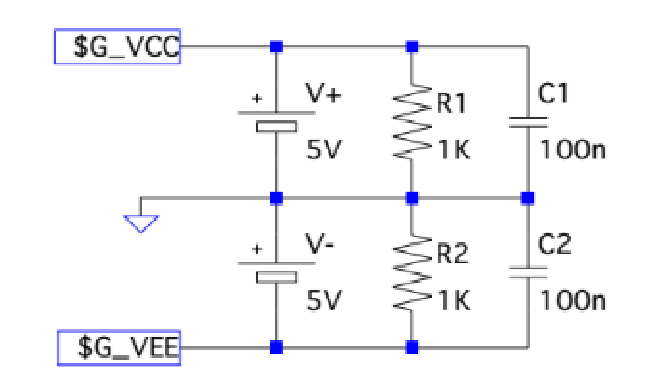
\includegraphics[width=0.6\textwidth]{prelim.png}
			\caption{Circuito di filtro per l'alimentazione.}
			\label{fig:prel}
		\end{minipage}
		\begin{minipage}{0.3\textwidth}
			\begin{tabular}{l@{ }c@{ }l}
				$R_{1}$& = &\SI{9.84(9)}{\kilo\ohm}\\
				$R_{2}$& = &\SI{9.74(9)}{\kilo\ohm}\\
				$C_1$& = &\SI{113(5)}{\nano\farad}\\
				$C_2$& = &\SI{106(5)}{\nano\farad}\\
			\end{tabular}
		\end{minipage}
	\end{figure}

\section{Metodo di misura}	 

	Per effettuare le misure è stato realizzato l'apparato in \figurename{ \ref{fig:completo}}
	verificando per ciascuno dei blocchi in figura l'operatività.
	Effettuate tali verifiche sono stati collegati tra loro i vari blocchi
	e sono stati acquisiti i valori di tensione, $V_{RMS}$, letti in continua sul voltmetro,
	per vari valori di resistenze in dotazione.

	Dalla campionatura ottenuta attraverso un fit a tre parametri sono state ottenuti i valori
	di $V_{0n}$, $R_{T}$, $R_{n}$; rispettivamente : il rumore in uscita a resistenza nulla; la resistenza equivalente del rumore serie dell'amplificatore riferito all'ingresso ed il rapporto tra il rumore parallelo; il rumore serie dell’amplificatore, riferiti all’ingresso.

	\begin{figure}[h]
			\centering
			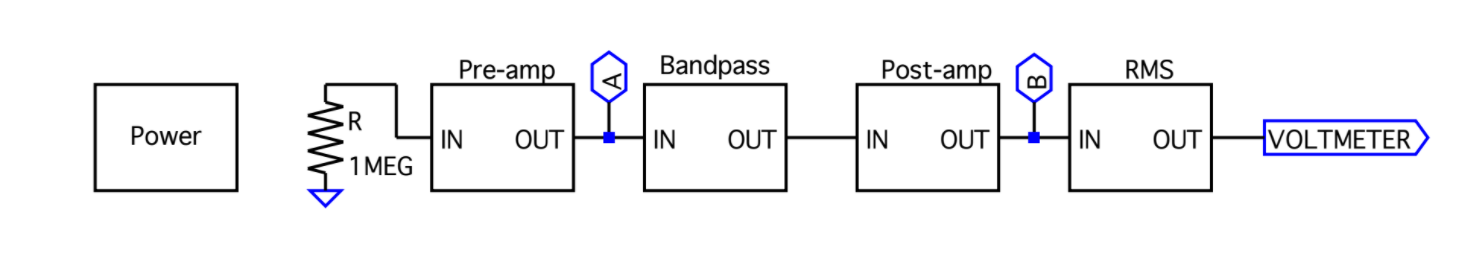
\includegraphics[scale = 0.5]{completo.png}
			\caption{schema dell'apparato di misura.}
			\label{fig:completo}
	\end{figure}

	Tali valori, essendo determinati da $k_{B}$ da relazioni descritte nel seguito, hanno permesso
	di ricavare una misura della costante di Boltzmann. 

\section{Pre-amplificatore}
	Il pre-amplificatore è realizzato dal circuito in \fig{pre}.

	\begin{figure}[h]
		\begin{minipage}{0.75\textwidth}
			\centering
			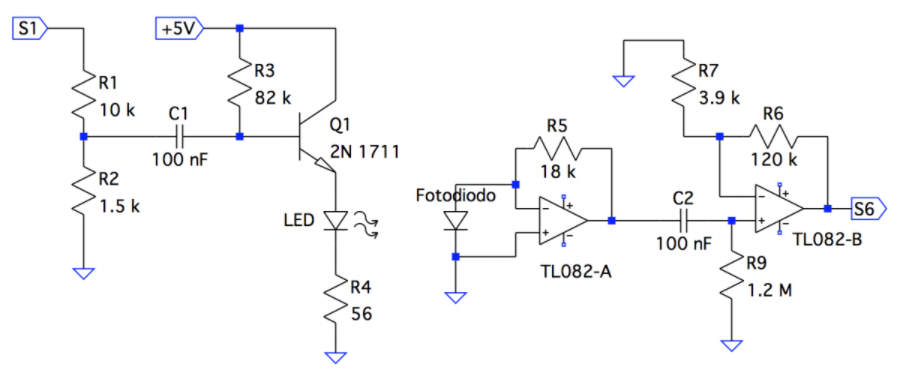
\includegraphics[width=\textwidth]{ampli.png}
			\caption{Circuito pre-amplificatore.}
			\label{fig:pre}
		\end{minipage}
		\begin{minipage}{0.19\textwidth}
			\begin{tabular}{l@{ }c@{ }l}
				$R_{1}$& = &\SI{0.971(9)}{\kilo\ohm}\\
				$R_{2}$& = &\SI{4.69(5)}{\kilo\ohm}\\
				$R_3$& = &\SI{71.9(7)}{\kilo\ohm}\\
			\end{tabular}
		\end{minipage}
	\end{figure}

	Essendo il guadagno atteso in $out$ $\sim 51 \cdot 14.5 \sim 740$, per effettuare
	la verifica evitando che l'uscita degli OpAmp saturi senza dover inviare segnali molto piccoli e dunque relativamente molto rumorosi
	si è scelto di valutare separatamente l'amplificazione delle due sezioni; è
	inoltre stato montato un partitore di tensione (impiegando le resistenze $R_{T1}=\SI{0.987(9)}{\kilo\ohm}$ e $R_{T2}=\SI{1031(9)}{\kilo\ohm}$) per valutare più agevolmente l'amplificazione della prima sezione.

	Si è proceduto pertanto ad inviare in ingresso al partitore un onda sinusoidale di varie ampiezze, misurando l'ampiezza dell'onda in uscita all'INA114.

	Il guadagno ottenuto $A_{1} = \num{54.8(4)}$ si discosta dall'atteso $1 + \longfrac[2pt]{\SI{50}{\kohm}}{R_1} = 52.5$, ma il datasheet dell'OpAmp non riporta l'errore sul parametro di \SI{50}{\kohm} indicato, dunque non possiamo dire se rientri o meno nell'incertezza.

	Effettuata questa prima verifica si è proceduto a verificare il guadagno della seconda
	parte del circuito montato.
	Essendo i due circuiti indipendenti si sono di nuovo inviati direttamente alla resistenza $R_2$ segnali sinusoidali generati esternamente anzichè collegarvi l'output del precedente OpAmp.

	Si è misurato un guadagno $A_2=\num{15.50(1)}$, compatibile col valore atteso $\longfrac[2pt]{R_3}{R_2} = \num{15.33(18)}$.


	\begin{figure}[h]
		\centering
		\subfloat[Prima sezione, INA114.]{
			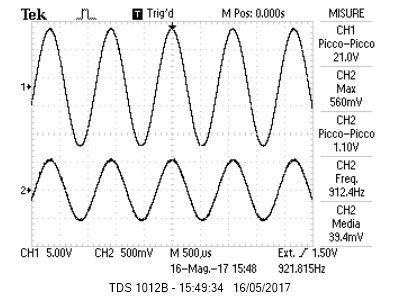
\includegraphics[scale=0.6]{preamp1.png}
		}
		\qquad
		\subfloat[Seconda sezione, AD708.]{
			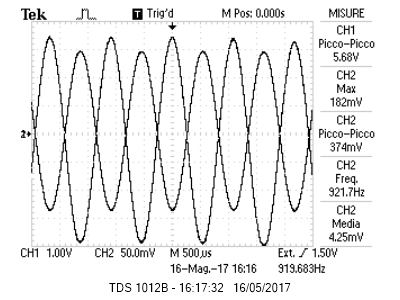
\includegraphics[scale=0.6]{preampb.png}
		}
		\caption{Acquisizioni esemplificative di segnali in ingresso (ch. 1) e in uscita (ch. 2).}
		\label{fig:preampo}
	\end{figure}

\section{Adattamento di fase}

Si è realizzato il circuito in \fig{sfas_circ}, che ha in ultima analisi lo scopo di generare un'onda approssimativamente quadra della stessa frequenza del segnale inviato al LED e che abbia con esso una precisa relazione di fase.

\begin{figure}[h]
	\begin{minipage}{0.75\textwidth}
		\centering
		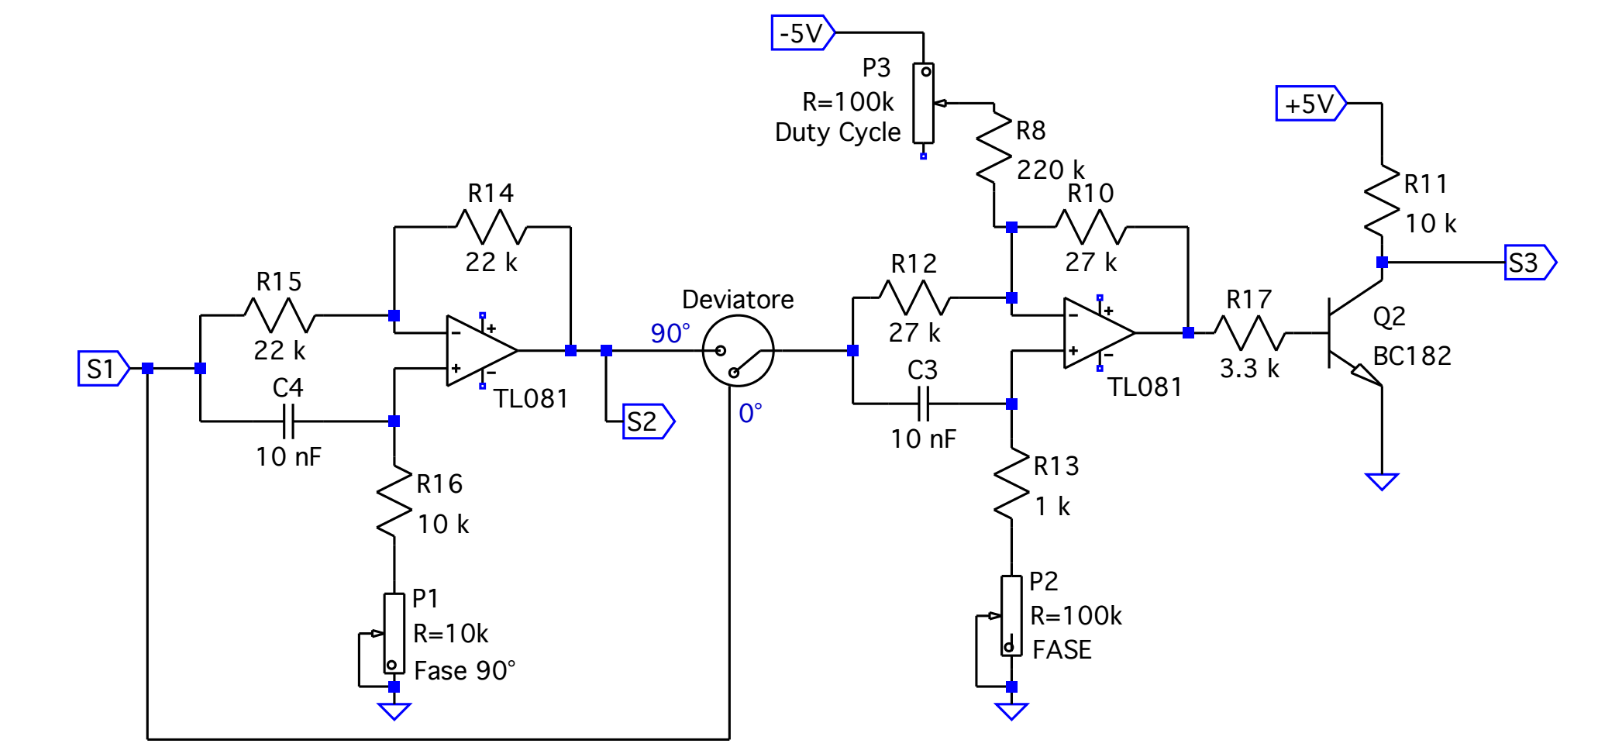
\includegraphics[width=\textwidth]{sfaso.png}
		\caption{Circuiti sfasatori (\ang{90} e fase variabile).}
		\label{fig:sfas_circ}
	\end{minipage}
	\begin{minipage}{0.19\textwidth}
		\begin{tabular}{l@{ }c@{ }l}
			$R_{8}$& = &\SI{217(3)}{\kilo\ohm}\\
			$R_{10}$& = &\SI{26.6(3)}{\kilo\ohm}\\
			$R_{11}$& = &\SI{9.95(9)}{\kilo\ohm}\\
			$R_{12}$& = &\SI{26.6(4)}{\kilo\ohm}\\
			$R_{13}$& = &\SI{979(9)}{\ohm}\\
			$R_{14}$& = &\SI{21.7(3)}{\kilo\ohm}\\
			$R_{15}$& = &\SI{21.4(3)}{\kilo\ohm}\\
			$R_{16}$& = &\SI{9.82(9)}{\kilo\ohm}\\
			$R_{17}$& = &\SI{3.25(3)}{\kilo\ohm}\\
			$C_3$& = &\SI{11.4(5)}{\nano\farad}\\
			$C_4$& = &\SI{11.2(5)}{\nano\farad}
		\end{tabular}
	\end{minipage}
\end{figure}

\subsection{Sfasatore di \ang{90}}

Si vuole che la prima sezione del circuito (quella precedente al deviatore) introduca uno sfasamento di $\SI{\pi/2}{rad}$ nel segnale in ingresso; la sua funzione di trasferimento (determinata col metodo del cortocircuito virtuale) è:
$$ V_{S2} = \longfrac{j \omega C_4 (P_1 + R_{16}) R_{14} / R_{15} - 1}{j \omega C_4 (P_1 + R_{16}) + 1} \ V_{S1}  $$
Dove $P_1$ rappresenta l'effettiva resistenza nel potenziometro nella posizione usata.
La differenza di fase tra ingresso e uscita vale dunque:
$$ \phi_{S2} - \phi_{S1} = \Delta\phi_1 = \pi - \atan \left( \omega  C_4 (P_1 + R_{16}) \frac{R_{14}}{R_{15}} \right) - \atan\mathopen{}\big( \omega C_4 (P_1 + R_{16}) \mathclose{}\big)$$
Ed è dunque decrescente dal suo valore massimo al crescere di $P_1$. Si è pertanto proceduto a regolare il potenziometro ottenendo una differenza temporale tra $S1$ ed $S2$ pari a \SI{244(2)}{\us}, che alla frequenza di lavoro di \SI{1.026(2)}{\kHz} corrisponde ad una differenza di fase di \SI{0.498(4)}{\pie.rad}.

\subsection{Sfasatore a fase variabile e transistor NOT}

La seconda parte del circuito intende nuovamente sfruttare un OpAmp per introdurre una differenza di fase ed inoltre un offset; l'output dell'OpAmp andrà (attraverso una resistenza per limitare il flusso di corrente) alla base di un transistor BJT in configurazione common emitter, il quale ha essenzialmente un comportamento da NOT gate: l'offset è necessario per compensare la tensione di soglia (positiva) per la commutazione del transistor e permetterci di ottenere un duty cicle del \SI{50}{\percent}.

La relazione tra ingresso e uscita del circuito è:

$$ V_{out} = \longfrac{j \omega C_3 (P_2 + R_{13}) R_{10} \big(1/R_{12} + 1/(R_8 + P_3)\big) - 1}{j \omega C_3 (P_2 + R_{13}) + 1} \, V_{in} + \longfrac{R_{10}}{R_8 + P_3} \, \SI{5}{\V}$$

Dove $V_{in}$ è la tensione in corrispondenza del deviatore, $V_{out}$ la tensione in uscita all'OpAmp e $P_2$ e $P_3$ sono le effettive resistenze dei potenziometri nelle posizioni usate.

Si è dunque variato $P_3$ in modo da ottenere in $S3$ un'onda quadra con $T_{up} = \SI{484(4)}{\us}$, essenzialmente pari alla metà del periodo dell'onda (\SI{987(8)}{\us}), riportata in \fig{duty_quadra}.

\begin{figure}[h]
	\centering
	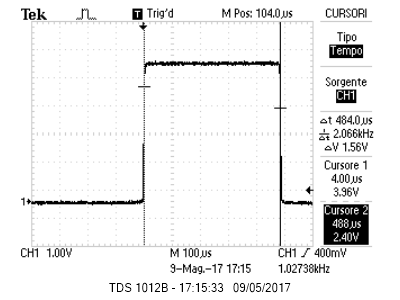
\includegraphics[scale=0.6]{duty_cycle.png}
	\caption{Segnale in uscita in $S3$.}
	\label{fig:duty_quadra}
\end{figure}

Variando $P_2$ è possibile variare la differenza di fase tra ingresso è uscita (cosa che servirà a compensare differenze di fase introdotte dal resto del circuito), ottenendo alle posizioni estreme del potenziometro:
\begin{center}
	$\Delta\phi_{2,min} = \SI{0.0468(4)}{\pie rad}$ \qquad e \qquad $\Delta\phi_{2,max} = \SI{0.915(8)}{\pie rad}$
\end{center}

Tale intervallo si è in seguito rivelato insufficiente per ottenere un segnale nullo al mediatore (ci saremmo dovuti avvicinare maggiormente a 0 o a \si{\pie rad}) ed è stato necessario introdurre un'ulteriore resistenza in serie al potenziometro ($\approx\SI{330}{\kilo\ohm}$) per ovviare al problema.

Il deviatore ci permette di avere in ingresso in quest'ultima sezione del circuito alternativamente il segnale inviato al LED oppure il segnale in uscita allo sfasatore di \ang{90}, consentendoci di introdurre a comando uno sfasamento di $\SI{\pi/2}{rad}$ nel segnale in uscita, come mostrato in \fig{devianza}, cosa che sarà necessaria nel seguito dell'esperienza.

\begin{figure}[h]
	\centering
	\subfloat[Deviatore verso $S2$]{
		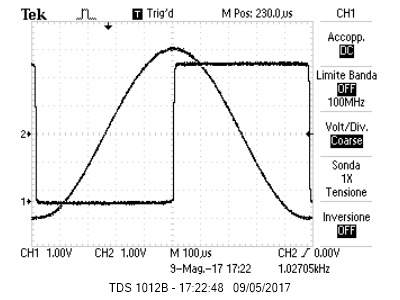
\includegraphics[scale=0.5]{deviatore1.png}
	}
	\qquad
	\subfloat[Deviatore verso $S1$]{
		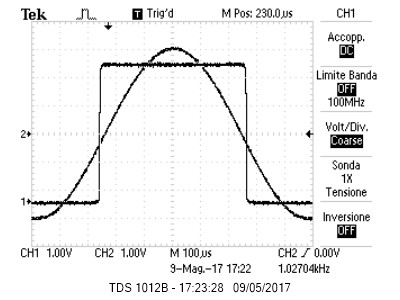
\includegraphics[scale=0.5]{deviatore2.png}
	}
	\caption{Segnali in ingresso ($S1$, ch. 2) e uscita ($S3$, ch. 1) nelle due posizioni del deviatore.}
	\label{fig:devianza}
\end{figure}

\section{Squadratore e campionatore}
	Dopo aver effettuato le verifiche precedenti è stato montato il 
	circuito in 
	\figurename{ \ref{fig:sqd} }
	impiegando le componenti circuitali corrispondenti.
	
	\begin{figure}[ht]
		\centering
		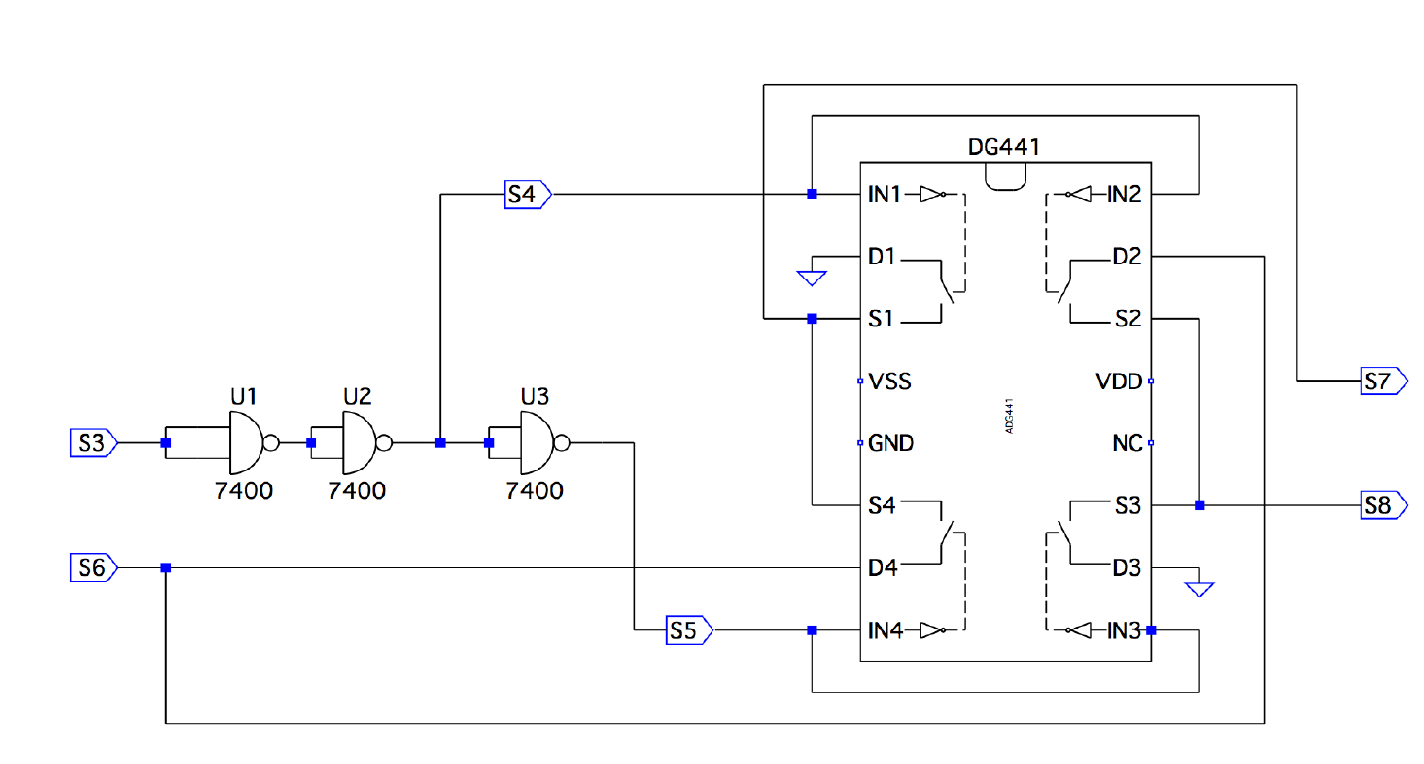
\includegraphics[scale=0.25]{deriv.png}
		\caption{Circuito che svolge la funzione di squadratore e campionatore}
		\label{fig:sqd}
	\end{figure}

	Il circuito costruito svolge la funzione di squadrare e campionatore la tensioni immesse.
	
	Si è proceduto pertanto alla verifica del funzionamento circuitale.
	Sono state d'apprima acquisite le forme d'onda visualizzabili su $S4-S5$
	ottenendo come da attese due segnali in opposizione di fase.
	\figurename{ \ref{f:s4-s5} }
	
	\begin{figure}[ht]
		\centering
		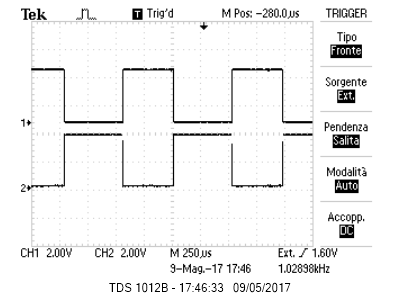
\includegraphics[scale=0.35]{s4-s5.png}
		\caption{segnale su s4 ch.1, s5 ch.2 }
		\label{f:s4-s5}
	\end{figure}
	
	Dopodiché sono stati acquisiti i segnali visualizzabili sui terminali $S7$ e $S8$
	per le due diverse posizioni del deviatore.
	
	Come è possibile vedere dalla \figurename{\ref{fig:s7}} si ottiene che i due segnali, qualora il
	deviatore sia collegato ad $S2$,  risultino dovuti alle semi-onda
	positiva o negativa, a seconda della traccia in esame.
	
	Per il deviatore collegato ad $S1$
	si attendono invece segnali a media nulla; le tracce ottenute risulta in buon accordo 
	con le attese.
	
	La presenza di spike in \figurename{\ref{fig:S7a}} e la non perfetta corrispondenza della media dei segnali a $0$ in \figurename{\ref{fig:S7b}} è stata imputata alla non idealità 
	degli operazionali impiegati nei montaggi circuitali.
	\begin{figure}[h]
		\centering
		\subfloat[ch.1 S7 ch.2 S8. Deviatore collegato a $S2$ ]{
			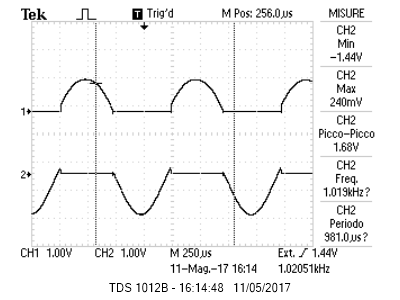
\includegraphics[scale=0.45]{s7-s8a.png}
			\label{fig:S7a}
		}
		\subfloat[ch.1 S7 ch.2 S8. Deviatore collegato ad $S1$]{
			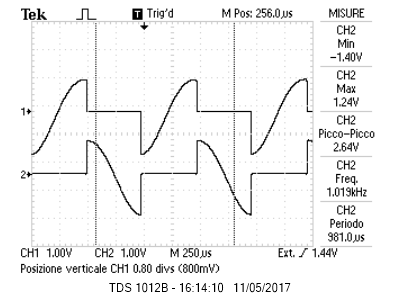
\includegraphics[scale=0.45]{s7-s8b.png}
			\label{fig:S7b}
		}
		\caption{Segnali acquisiti di $S7-S8$}
		\label{fig:s7}
	\end{figure}

\end{document}
